\documentclass[final,t]{beamer}

% poster template
\usepackage[orientation=portrait,size=a0,scale=1.4,debug]{beamerposter}
\usetheme{zurichposter}
\usepackage{graphicx}
\usepackage{varwidth}
\usepackage{multirow}
% references
%\usepackage[bibstyle=authoryear, citestyle=authoryear-comp,%
%hyperref=auto]{biblatex}
%\bibliography{references}

\newcommand*\circled[1]{\tikz[baseline=(char.base)]{
            \node[shape=circle,draw,inner sep=2pt] (char) {#1};}}
%title

% document properties
\title{\LARGE HAShCache: Heterogeneity Aware Shared DRAMCache For Integrated Heterogenous Architectures}
\author{Adarsh Patil, R Govindarajan}
\institute{Department of CSA, Indian Institute of Science, Bangalore }


%------------------------------------------------------------------------------
\begin{document}

% my figures
\input{../figures}

\begin{frame}[t,fragile]{}

% gloablly set small font
\small

%-----------------------------------------------------------------------------
%                                                                     COLUMN 1
% ----------------------------------------------------------------------------

%+++++++++++++++++++++++++++++++++++++++++++++++++++++++++++++++++++++++++++++    

    % intro D$
    \vspace{1.5em}
    \begin{tcolorbox}[colback=red!5!white,
                      colframe=red!75!black,
                     ]
        \begin{columns}[t]
        \begin{column}{.48\linewidth}
       
            \begin{exampleblock}{Integrated Heterogenous Systems (IHS) Architecture}

        	\begin{itemize}
    	    	\item \textit{Throughput-oriented} GPGPU SMs + \textit{Latency-oriented} CPU cores on-chip
       			\item Shared Physical/Virtual Address Space and a Unified Memory Hierarchy 
    			%\item Cache Coherent Interconnect
    	    	\item Improved Programmability
    			\item AMD APUs, Intel Iris, NVIDIA Denver
    	        \end{itemize}    
    		\begin{figure}
    			\centering
    			\def\svgwidth{0.7\linewidth}
    			\input{arch.pdf_tex} 
    		\end{figure}
            \end{exampleblock}
     \end{column}
     \begin{column}{.48\linewidth}
        \begin{exampleblock}{Vertically Stacked DRAM}
            	\centering DRAM Layers stacked using 2.5D interposer or 3D TSV
\vspace{1.5em}
\begin{table}[]
\centering
\setlength{\tabcolsep}{1em}
\begin{tabular}{lll}
             & \textbf{Stacked DRAM}                                                     & \textbf{Off-chip DRAM} \\
             \hline
Capacity     & $\sim$ 64MB - 4GB                                                         & $\sim$ 4GB - 128GB     \\
Bandwidth    & $\sim$ 500GB/s                                                            & $\sim$ 90 GB/s         \\
Latency      & $\sim$ 30ns - 35ns                                                        & $\sim$ 50ns            \\
Interconnect & TSV (through-silicon-vias)                                                & Memory Channels        \\
Standards    & $HBM_{(AMD/Hynix)}$, $HMC_{(Intel/Micron)}$ & DDR4. GDDR5           
\end{tabular}
\end{table}
\vspace{0.9em}
            		\begin{figure}
            			\centering
            			\def\svgwidth{0.62\linewidth}
            			\input{stackedDRAM.pdf_tex} 
            		\end{figure}
        \end{exampleblock}
      \end{column}
      \end{columns}
    \end{tcolorbox}

    
% ----------------------------------------------------------------------------        
\begin{columns}[t]

\begin{column}{.48\linewidth}
\begin{tcolorbox}[colback=red!5!white,
                  colframe=red!75!black,
                 ]
    % motivation
    \begin{exampleblock}{Motivation and Design}
    \centering 
    \underline{Performance}

    \begin{itemize}
      	%\item Effect of Co-running \\
      	%	\qquad - CPU performance severely degraded, drops 320\% from homogeneous CPU\\
      	%	\qquad - GPU remain relatively unaffected, drops 7\% from homogeneous GPU
      	\item Naive addition of DRAM\$ over IHS \\
      		\qquad - CPU performs 42\% better while Homogeneous CPU achieves 372\% improvement  \\
      		\qquad \qquad \emph{\color{red}2.6x performance gap}\\
      		\qquad - GPU performs 24\% better while Homogeneous GPU achieves 26.4\% improvement \\ 
      		\qquad \qquad \emph{10\% performance gap}\\
      	\item Un-managed interference and Heterogeneity in the DRAM\$
    \end{itemize}
    \begin{figure}
       \includegraphics[scale=2]{graphs/motivation-cpu}
    \end{figure}
    \begin{figure}
       \includegraphics[scale=2]{graphs/motivation-gpu}
       \caption{Performance comparison of CPU \& GPU in IHS with D\$ vs Homogeneous with D\$}
       \label{fig:motivation}
    \end{figure}
    
    \underline{Causes for sub-optimality of DRAM\$}
    \begin{itemize}
   		\item Increased DRAM\$ access times for CPU despite comparable hit rates
        \item Allow GPU to occupy enough cache to benefit from the large DRAM\$ bandwidth
    \end{itemize}
    
    \begin{figure}
       \includegraphics[scale=2.05]{graphs/motivation-cpu-cache}
       \includegraphics[scale=2.05]{graphs/motivation-gpu-cache}
       \caption{(a)CPU D\$ Access Latency and Hit Rates (b)GPU Misses with 2-way assoc cache}
       \label{fig:motivation-cpu-cache}
    \end{figure}  

\vspace{1em}
\begin{table}[]
\centering
\begin{tabular}{ll}
\textbf{Design Point}                   & \textbf{Design Decision}          \\
\hline
Metadata Overhead & Tags in DRAM, 128 Byte TAD (Tag-and-Data) Units        \\
Set Associativity                                           & Direct Mapped                                          \\
Miss Penalty                                                & Miss Predictor for CPU requests                        \\
Addressing Scheme                                           & Row-Rank-Bank-Column-Channel (RoRaBaCoCh)
\end{tabular}
\caption{HAShCache Design Decisions}
\end{table}
    \end{exampleblock}
     

%-----------------------------------------------------------------------------



%-----------------------------------------------------------------------------


%-----------------------------------------------------------------------------

%+++++++++++++++++++++++++++++++++++++++++++++++++++++++++++++++++++++++++++++
\end{tcolorbox}
\end{column}


%-----------------------------------------------------------------------------
%                                                                     COLUMN 2
% ----------------------------------------------------------------------------
\begin{column}{.48\linewidth}
\begin{tcolorbox}[
                  title={\vspace{0.7em} \large \ HAShCache \ = \ \textit{PrIS} \ + \ \textit{ByE} \ + \ \textit{Chaining} \vspace{0.4em}
                         },
                  colback=red!5!white,
                  colframe=red!75!black,
                  coltitle=red!25!black,
                  colbacktitle=yellow!50!red,	
                  fonttitle=\bfseries,
                 ]

%+++++++++++++++++++++++++++++++++++++++++++++++++++++++++++++++++++++++++++++

% ----------------------------------------------------------------------------   

    % Priority
    \begin{exampleblock}{ \circled{1} Hetereogenity Aware DRAM\$ Scheduling: PrIS}
    \begin{itemize}
    	\item \emph{OBJECTIVE:} Reduce large access latencies for CPU requests at DRAM\$
    	\item Large number of GPU requests $\implies$ queues fill up rapidly $\implies$ CPU request rejected
    	\item GPU requests have good row buffer locality $\implies$ preferentially scheduled $\implies$ large queuing latency for CPU requests
    	\item \emph{Achieved} using \\
    	\qquad - Queue entry reservation for CPU requests when queues reach critical levels \\
    	\qquad - CPU Prioritized FR-FCFS with IHS-aware scheduling algorithm
    \end{itemize} 
	\end{exampleblock}
	    
	\vspace{0.8em}
% ----------------------------------------------------------------------------    

    % bypass
    \begin{exampleblock}{\circled{2} Temporal Selective Bypass Enabler : \textit{ByE}}
    	\begin{columns} [T]
    		\begin{column}{0.6\linewidth}
    	    \begin{itemize}
    	    	\item \emph{OBJECTIVE:} Utilize the idle DRAM bandwidth
    	    	\item Bypass CPU requests to clean cache lines and cache misses
    	    	\item \emph{Achieved} using a \textit{Counting Bloom Filter} that tracks dirty lines in cache
    	    	\item Overhead: 256KB (0.4\% of cache capacity)
			    %\item Fig shows working of HAShCache + ByE
    	    \end{itemize}     			
    		\end{column}
    		\begin{column}{0.4\linewidth}
    			\begin{figure}
					\centering
            		\def\svgwidth{0.9\linewidth}
            		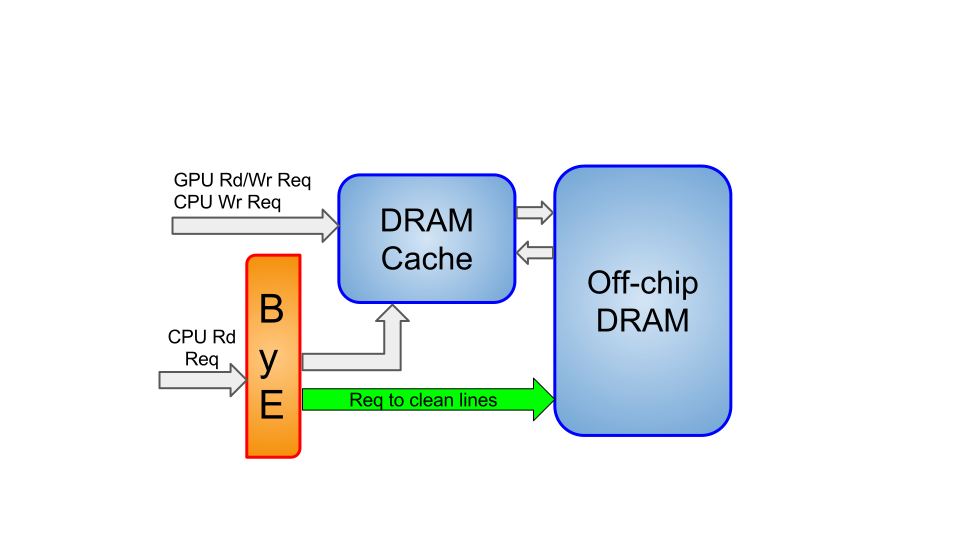
\includegraphics[scale=0.9]{bypass.png}
    			\end{figure}
    	    \end{column}
    	\end{columns}
	\end{exampleblock} 
    \vspace{0.8em}
% ----------------------------------------------------------------------------        

    % chaining
    \begin{exampleblock}{\circled{3} Spatial Occupancy Control : \textit{Chaining}}
    	\begin{itemize}
	    	\item \emph{OBJECTIVE:} Allow GPU to better use DRAM\$ bandwidth
		    \item \emph{Achieved} by providing pseudo-associativity for GPU, thus improving GPU hit rate
		    \item Provides guaranteed minimum occupancy for CPU lines in the cache
	    	\item GPU set conflicts resolved by evicting an adjoining "\textit{chained}" set belonging to the CPU
		    %\item Chaining done until minimum CPU occupancy threshold is reached
		    \item Overhead: NIL, uses unused bits in DRAM\$ rows
	    \end{itemize}
	\vspace{\baselineskip}
    \centering
    \begin{figure}
    	\centering
        \def\svgwidth{0.31\linewidth}
        %\input{chainings.pdf_tex}
        \hspace{0.4em}	
    	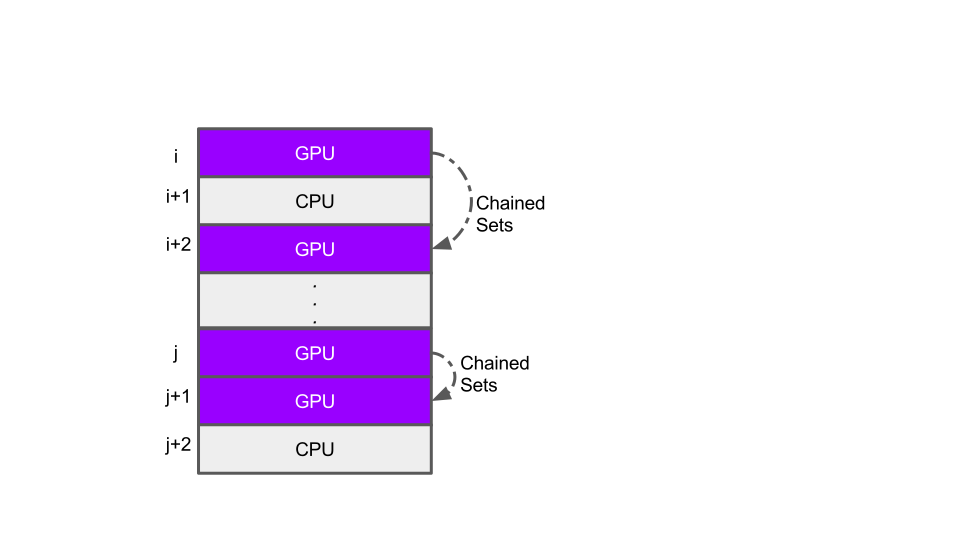
\includegraphics[scale=1.1]{chainings}
    	\caption{HAShCache Row Organization and Access Path of a request}
    \end{figure}
    \end{exampleblock}
          
% ----------------------------------------------------------------------------    

\end{tcolorbox}
\end{column}

\end{columns}

    \vspace{1.5em}
        \begin{tcolorbox}[colback=red!5!white,
                          colframe=red!75!black,
                         ]
        \begin{columns}[t]
        \begin{column}{.48\linewidth}
       
	
		\begin{exampleblock}{Results}
        	\begin{figure}
				\includegraphics[scale=2]{graphs/results-cpu}
			\end{figure}
			\begin{figure}
			   	\includegraphics[scale=2]{graphs/results-gpu}
		  	    \caption{Speedup obtained by HAShCache mechanisms for (a)CPU (b)GPU}
			\end{figure} 
		\end{exampleblock}
		
     \end{column}
     \begin{column}{.48\linewidth}
	\begin{exampleblock}{Conclusion}
	\begin{itemize}
	\item HAShCache  \quad - Heterogeneity aware organization \quad \ \  - improves IHS performance  \\ 
	  \qquad \qquad \qquad \ - achieves better resource utilization \quad- reduces energy consumed
	\item Compared to a heterogeneity unaware DRAM\$ (naive) \\
	\quad - \textit{Chaining} + \textit{PrIS} improves perf of CPU by 44\% by trading off just 6\% of GPU perf \\
	\quad - \textit{ByE} + \textit{PrIS} improves perf of CPU by 48\% while sacrificing just 3\% of GPU perf
	\item Overall, HAShCache improves system performance by \\ 
	       \qquad - {\color{red}41\%} over a naive DRAM\$ \\ 
	       \qquad - {\color{red}211\%} over the baseline system with no DRAM\$
	\end{itemize}
	
	\end{exampleblock}
	
		\footnotesize{*This work has been submitted to the  50th Annual IEEE/ACM International Symposium on Microarchitecture (MICRO-50) and is currently under review} \\
		\vspace{2em}
		\footnotesize{The authors can be contacted at adarsh.patil@csa.iisc.ernet.in / govind@csa.iisc.ernet.in}
      \end{column}
      \end{columns}
    \end{tcolorbox}

\end{frame}

\end{document}
